
\section{Die Entdeckung des Higgs-Bosons}

\chapterauthor{Patrick Schmidt, 11.01.2019}

\subsection{Geschichte und Theorie der spontanen Symmetriebrechung}
Die in den 1960er Jahren durch Glashow, Weinberg und Salam beschriebene elektroschwache Theorie zur vereinheitlichten Erklärung der elektromagnetischen und schwachen Wechselwirkung besaß bis ins Jahr 1964 keine Erklärung des Zustandekommens der Massen der dazugehörigen Eichbosonen.
Erst der durch Peter Higgs eingeführte Higgs-Mechanismus lieferte durch die Einführung eines skalaren Feldes eine mit Massen kompatible Theorie.

Grundlegend für den Higgs-Mechanismus ist das Phänomen der spontanen Symmetriebrechung, welches auch beispielsweise in der Festkörperphysik bei einem Ferromagneten beobachtet werden kann.
Ein einfaches Beispiel ist durch das in Abbildung \ref{fig:higgs} angegebene Potential gegeben.

\begin{figure}
  \centering
  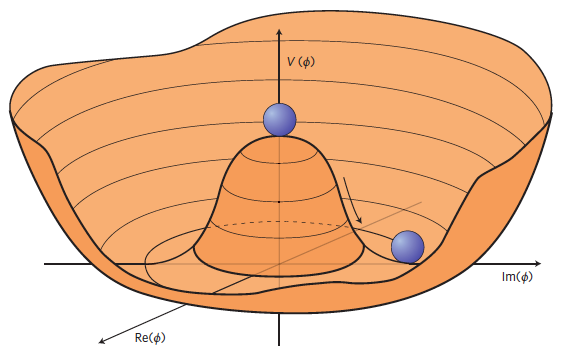
\includegraphics[height=5.0cm]{ressources/higgspotential.png}
  \caption{"Mexiko-Hut-Potential" als Beispiel zur spontanen Symmetriebrechung \cite{Ellis:2012465}}
  \label{fig:higgs}
\end{figure}

Hier ist das Minimum des Potentials vom Ursprung verschoben.
Gleichzeitig existieren mehrere, prinzipiell gleichberechtigte Minima, welche alle denselben Vakuumserwartungswert besitzen.
Die Wahl eines dieser Minima entspricht dabei der spontanen Symmetriebrechung, analog zur Wahl einer Vorzugsrichtung bei Abkühlung eines Ferromagnetens unter die Curie-Temperatur.
Der Lagrangian, welcher das oben beschriebene Potential verkörpert, kann nun um den neuen Vakuumerwartungswert betrachtet werden.
Hierbei tritt, wie durch das Goldstone-Theorem beschrieben, ein masseloses Goldstone-Boson auf.

Im Rahmen des Higgs-Mechanismus treten Wechselwirkungen zwischen deim Higgs-Feld sowie den Feldern der Eichbosonen auf.
Durch diese Kopplungsterme treten sowohl die massebehafteten Eichbosonen auf als auch deren Kopplung an das Higgs-Boson.
Die im Standardmodell gebrochene Symmetrie ist dabei die $SU(3) \times U(1)$-Symmetrie.

\subsection{Suche nach Singaturen des Higgs-Bosons}
Während der Higgs-Mechanismus zwar eine theoretische Erklärung der Massen der Eichbosonen liefert, würde nur ein tatsächlicher Nachweis des Higgs-Bosons dazu führen, dass ebendieser Mechanismus als korrekte Theorie bestätigt werden kann.
Bei der Betrachtung der infrage kommenden Erzeugungs- und Zerfallskanäle ist zu beachten, dass die auftretenden Kopplungen an das Higgs-Boson proportional zu den beteiligten Massen sind.
Ein möglicher Prozess zur Erzeugung sowie Zerfall unter Kopplung an das schwerste bekannte Quark, das Top-Quark, ist in Abbildung \ref{fig:higgs2} dargestellt.
Zu beachten ist, dass für verschiedene mögliche Massen des Higgs-Bosons verschiedene Zerfallskanäle dominieren können.
Bei späteren Analysen ist jedoch nicht immer die einzige Betrachtung des domnierenden Zerfallskanals sinnvoll, da häufig andere Untergrundprozesse (beispielsweise beim $\text{b}\overline{\text{b}})$-Kanal andere hadronische Prozesse) dominieren.

\begin{figure}
  \centering
  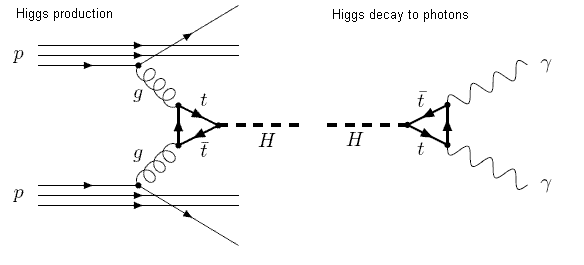
\includegraphics[height=5.0cm]{ressources/higgsfeyn.png}
  \caption{Mögliche Erzeugung und möglicher Zerfall eines Higgs-Bosons. Die Gluonen können beispielsweise aus Protonen in pp-Kollisionen stammen \cite{higgs_production_decay}.}
  \label{fig:higgs2}
\end{figure}

\subsection{Untere Grenzen auf die Higgs-Masse durch erste experimentelle Untersuchungen}
Vor der finalen Entdeckung des Higgs-Bosons im Jahre 2012 konnten viele andere Experimente bereits Einschränkungen auf die Masse eines möglichen Higgs-Bosons treffen.

%TODO: BB_BAR Oszillationen?! 

Das Experiment NA31, welches von 1987 bis 1989 Messungen am SPS am CERN durchführte, hatte die primäte Aufgabe nach CP-Verletzung im Kaonsektor zu suchen.
Trotzdem konnte die Betrachtung der Daten unter Berücksichtigung eines möglichem Kaonzerfalls der Form
\begin{align*}
	\text{K}_\text{L}^0 \rightarrow \pi^0 \text{H}^0 \rightarrow \pi^0 e^+ e^-
\end{align*}
eine erste untere Grenze von $m_\text{H} = \SI{15}{\mega\electronvolt}$ angegeben werden.

Der LEP war ein $e^+ e^-$-Collider, welcher von 1989 bis 2000 betrieben wurde und Higgs-Bosonen über den Prozess
\begin{align*}
	e^+ e^+ \rightarrow \text{H} Z^0
\end{align*}
produzieren sollte.
Als Kanäle zur Beobachtung wurden als mögliche Endzustände 4-Jet-Zustände, Kanäle mit fehlender Energie aufgrund von zwei Neutrinos sowie leptonische Kanäle mit zwei Elektronen im Endzustand gesucht.
Zwar ergab die Suche keinen Erfolg, auf die Masse konnte jedoch ein unteres Limit von \SI{114.4}{\giga\electronvolt} gesetzt werden.

Mit den Experimenten D0 und CDF am Tevatron wurde in Daten von 2001 bis 2011 erstmals an einem $p\overline{p}$-Collider nach Higgs-Bosonen gesucht.
Hierbei kommt zur Produktion erstmals auch der in Abbildung \ref{fig:higgs2} dargestellte Kanal in Frage.
Das Experiment konnte dabei die Bereiche
\begin{align*}
	\SI{100}{\giga\electronvolt} &\leq m_\text{H} \leq \SI{108}{\giga\electronvolt} \\
	\SI{156}{\giga\electronvolt} &\leq m_\text{H} \leq \SI{177}{\giga\electronvolt} \\
\end{align*}
für die Higgs-Masse ausschließen.

\subsection{Entdeckung des Higgs-Bosons am LHC}

Studien über die Erzeugung von Higgs-Bosonen in $p\overline{p}$-Kollisionen in den 90er Jahren stellten die Grundlagen für den Bau des Large Hadron Colliders dar.
Auf Basis der durchgeführten Berechnungen wurden die Zerfallskanäle
\begin{align*}
	&\text{H} \rightarrow \gamma \gamma \\
	&\text{H} \rightarrow l^+ l^- l^+ l^- 
\end{align*}
als relevanteste Kanäle zur Detektion bei der Konstruktion des Detektoren berücksichtigt.

Nach dem ersten Betriebsbeginn im September 2008 mit einem anschließenden Betriebsstop aufgrund von nötigen Reparaturen konnte am 2010 mit Messungen bei einer Schwerpunktsenergie von $\sqrt{s} = \SI{7}{\tera\electronvolt}$ begonnen werden.
Erste Analyseergebnisse in den oben angegebenen Kanälen konnten die Masse auf einen Bereich 
\begin{align*}
	\SI{115.5}{\giga\electronvolt} &\leq m_\text{H} \leq \SI{131}{\giga\electronvolt}
\end{align*}
einschränken.

Nachdem die Schwerpunktsenergie 2012 auf \SI{8}{\giga\electronvolt} erhöht und somit die Higgs-Produktion gesteigert weden konnte ergaben sich erste Hinweise in den Daten rund um \SI{125}{\giga\electronvolt}.
Am 4. Juli 2012 gaben die beiden Detektorexperimente ATLAS und CMS einen Ausschlag in den Daten bei
\begin{align*}
  m_{\text{H, ATLAS}} &= \left( \num{126.0} \pm \num{0.4} \pm \num{0.4} \right) \si{\giga\electronvolt} \\
  m_{\text{H, CMS}} &= \left( \num{125.3} \pm \num{0.4} \pm \num{0.5} \right) \si{\giga\electronvolt}
\end{align*}
bekannt.

Die Analyse am ATLAS Experiment wurde über die Kanäle
\begin{align*}
  &\text{H} \rightarrow Z Z^* \rightarrow 4l \\
  &\text{H} \rightarrow \gamma \gamma \\
  &\text{H} \rightarrow W W^* \rightarrow e \nu \mu \nu
\end{align*}
durchgeführt.
Der Kanal mit zwei Photonen im Endzustand war dabei insbesondere im Bereich von \SI{110}{\giga\electronvolt} bis \SI{150}{\giga\electronvolt} sentitiv, wobei insbesondere Untergründe aus Z-Produktion bzw. Pionzerfällen berücksichtigt werden mussten.
Ebenfalls musste berücksichtigt werden, inwiefern Jets ggf. als Phontonen falsch rekonstruiert wurden.
Unter Betrachtung der beiden Photonen mit größtem $p_\text{T}$ konnte, unter Betrachtung der Energieeinträge in den elektromagnetischen Kalorimetern, die invariante Masse rekonstruiert und somit ein Rückschluss auf die Higgsmasse gezogen werden.

Am CMS wurden eben den oben genannten Kanälen zusätzlich die Kanäle 
\begin{align*}
  &\text{H} \rightarrow \tau^+ \tau^- \\
  &\text{H} \rightarrow \text{b} \overline{\text{b}} \rightarrow 2 \text{Jets}
\end{align*}
betrachtet.
Bei der Betrachtung der Kanäle mit vier Leptonen im Endzustand ist zu beachten, dass die Leptonenpaare jeweils aus demselben primären Vertex stammen.
Zudem muss gewährleistet sein, dass die Myonen bzw. Elektronen isoliert als Paare auftreten.
Als Untergründe sind insbesondere entstehende Z-Bosonen aus $\text{q}\overline{\text{q}}$-Produktion sowie als Leptonen identifizierte Photonen zu berücksichtigen.

Für die Entdeckung des Higgs-Bosons erhielten F. Englert und P. Higgs im Jahre 2013 den Nobelpreis.

\subsection{Experimentelle Untersuchungen nach der Entdeckung}
Nach der Entdeckung des Higgs-Bosons wurden weitere Messungen zur Untersuchung der Eigenschaften durchgeführt.
Hierzu gehören insbesondere Messungen von Spin und Parität, welche zu $J^P = 0^+$ bestimmt werden konnten.
Die Spinmessung steht dabei insbesondere im Zusammenhang mit dem Landau-Yang-Theorem, da laut diesem ein Zerfall eines Teilchens mit Spin 1 in zwei Teilchen mit Spin 1 unterdrückt ist.
Dies würde sich auf den Zerfalls des Higgs in zwei Photonen auswirken.

Zudem wurden die genauen Kopplungen des Higgs genauer untersucht. 
Dies ist insbesondere deshalb von großer Bedeutung, da durch die Kopplung des Higgs an massereiche Teilchen eine Untersuchung von möglicher BSM-Physik sehr gut ermöglicht wird.
